\documentclass{article}
%\documentstyle[11pt,handout,psfig]{article}

\usepackage{fullpage,amssymb,amsmath,epsf, color}

\usepackage[12pt]{extsizes}
\usepackage{algorithm}
%These give really tight margins:
%\setlength{\topmargin}{-0.3in}
%\setlength{\textheight}{8.10in}
%\setlength{\textwidth}{5.8in}
%\setlength{\baselineskip}{0.1875in}
%\addtolength{\leftmargin}{-2.775in}
%\setlength{\footskip}{0.45in}
%\setlength{\oddsidemargin}{0.5in}
%\setlength{\evensidemargin}{0.5in}
%%\setlength{\headsep}{0pt}
%%\setlength{\headheight}{0pt}

%\setlength{\topmargin}{-0.5in}
\setlength{\textheight}{8in}
%\setlength{\textwidth}{5.0in}
%\setlength{\baselineskip}{0.1875in}
%\addtolength{\leftmargin}{-2.775in}
%\setlength{\footskip}{0.45in}
%\setlength{\oddsidemargin}{0.5in}
%\setlength{\evensidemargin}{0.5in}
%%\setlength{\headsep}{0pt}
%%\setlength{\headheight}{0pt}


\def\shownotes{1}  %set 1 to show author notes
\ifnum\shownotes=1
\newcommand{\authnote}[2]{$\ll$\textsf{\footnotesize #1 notes: #2}$\gg$}
\else
\newcommand{\authnote}[2]{}
\fi

\newcommand{\Tnote}[1]{{\color{blue}\authnote{Tengyu}{#1}}}

\newcommand{\notes}[1]{{\color{blue} Note:} \textit{#1} \newline}

\usepackage{graphicx}

%\renewcommand{\epsffile}[1]{
%	\includegraphics[width=\epsfxsize]{#1}
%}

\newcommand{\di}{{d}}
\newcommand{\nexp}{{n}}
\newcommand{\vcd}{{\textbf{D}}}


\markright{XCS229i}
\pagestyle{myheadings}

\newcommand{\newsec}{\section}
\newcommand{\denselist}{\itemsep 0pt\partopsep 0pt}
\newcommand{\bitem}{\begin{itemize}\denselist}
\newcommand{\eitem}{\end{itemize}}
\newcommand{\benum}{\begin{enumerate}\denselist}
\newcommand{\eenum}{\end{enumerate}}

\newcommand{\fig}[1]{\private{\begin{center}
{\Large\bf ({#1})}
\end{center}}}

\newcommand{\cpsf}[1]{{\centerline{\psfig{#1}}}}
\newcommand{\mytitle}[1]{\centerline{\LARGE\bf #1}}

\newcommand{\myw}{{\bf w}}

\newcommand{\mypar}[1]{\vspace{1ex}\noindent{\bf {#1}}}

\def\thmcolon{\hspace{-.85em} {\bf :} }

\newtheorem{THEOREM}{Theorem}[section]
\newenvironment{theorem}{\begin{THEOREM} \thmcolon }%
                        {\end{THEOREM}}
\newtheorem{LEMMA}[THEOREM]{Lemma}
\newenvironment{lemma}{\begin{LEMMA} \thmcolon }%
                      {\end{LEMMA}}
\newtheorem{COROLLARY}[THEOREM]{Corollary}
\newenvironment{corollary}{\begin{COROLLARY} \thmcolon }%
                          {\end{COROLLARY}}
\newtheorem{PROPOSITION}[THEOREM]{Proposition}
\newenvironment{proposition}{\begin{PROPOSITION} \thmcolon }%
                            {\end{PROPOSITION}}
\newtheorem{DEFINITION}[THEOREM]{Definition}
\newenvironment{definition}{\begin{DEFINITION} \thmcolon \rm}%
                            {\end{DEFINITION}}
\newtheorem{CLAIM}[THEOREM]{Claim}
\newenvironment{claim}{\begin{CLAIM} \thmcolon \rm}%
                            {\end{CLAIM}}
\newtheorem{EXAMPLE}[THEOREM]{Example}
\newenvironment{example}{\begin{EXAMPLE} \thmcolon \rm}%
                            {\end{EXAMPLE}}
\newtheorem{REMARK}[THEOREM]{Remark}
\newenvironment{remark}{\begin{REMARK} \thmcolon \rm}%
                            {\end{REMARK}}
%\newenvironment{proof}{\noindent {\bf Proof:} \hspace{.677e\nexp}}%
%                      {}

%theorem
\newcommand{\thm}{\begin{theore\nexp}}
%lemma
\newcommand{\lem}{\begin{lemma}}
%proposition
\newcommand{\pro}{\begin{propositio\di}}
%definition
\newcommand{\dfn}{\begin{definitio\di}}
%remark
\newcommand{\rem}{\begin{remark}}
%example
\newcommand{\xam}{\begin{example}}
%corollary
\newcommand{\cor}{\begin{corollary}}
%proof
\newcommand{\prf}{\noindent{\bf Proof:} }
%end theorem
\newcommand{\ethm}{\end{theore\nexp}}
%end lemma
\newcommand{\elem}{\end{lemma}}
%end proposition
\newcommand{\epro}{\end{propositio\di}}
%end definition
\newcommand{\edfn}{\bbox\end{definitio\di}}
%end remark
\newcommand{\erem}{\bbox\end{remark}}
%end example
\newcommand{\exam}{\bbox\end{example}}
%end corollary
\newcommand{\ecor}{\end{corollary}}
%end proof
\newcommand{\eprf}{\bbox\vspace{0.1i\di}}
%begin equation
\newcommand{\beqn}{\begin{equatio\di}}
%end equation
\newcommand{\eeqn}{\end{equatio\di}}

%\newcommand{\eqref}[1]{Eq.~\ref{#1}}

\newcommand{\KB}{\mbox{\it KB\/}}
\newcommand{\infers}{\vdash}
\newcommand{\sat}{\models}
\newcommand{\bbox}{\vrule height7pt width4pt depth1pt}

\newcommand{\act}[1]{\stackrel{{#1}}{\rightarrow}}
\newcommand{\at}[1]{^{(#1)}}

\newcommand{\argmax}{{\rm argmax}}

\newcommand{\rimp}{\Rightarrow}
\newcommand{\dimp}{\Leftrightarrow}

\newcommand{\bX}{\mbox{\boldmath $X$}}
\newcommand{\bY}{\mbox{\boldmath $Y$}}
\newcommand{\bZ}{\mbox{\boldmath $Z$}}
\newcommand{\bU}{\mbox{\boldmath $U$}}
\newcommand{\bE}{\mbox{\boldmath $E$}}
\newcommand{\bx}{\mbox{\boldmath $x$}}
\newcommand{\be}{\mbox{\boldmath $e$}}
\newcommand{\by}{\mbox{\boldmath $y$}}
\newcommand{\bz}{\mbox{\boldmath $z$}}
\newcommand{\bu}{\mbox{\boldmath $u$}}
\newcommand{\bd}{\mbox{\boldmath $d$}}
\newcommand{\smbx}{\mbox{\boldmath $\scriptstyle x$}}
\newcommand{\smbd}{\mbox{\boldmath $\scriptstyle d$}}
\newcommand{\smby}{\mbox{\boldmath $\scriptstyle y$}}
\newcommand{\smbe}{\mbox{\boldmath $\scriptstyle e$}}

\newcommand{\Parents}{\mbox{\it Parents\/}}
\newcommand{\B}{{\cal B}}
\newcommand{\calH}{{\cal H}}

\newcommand{\word}[1]{\mbox{\it #1\/}}
\newcommand{\Action}{\word{Actio\di}}
\newcommand{\Proposition}{\word{Propositio\di}}
\newcommand{\true}{\word{true}}
\newcommand{\false}{\word{false}}
\newcommand{\Pre}{\word{Pre}}
\newcommand{\Add}{\word{Add}}
\newcommand{\Del}{\word{Del}}
\newcommand{\Result}{\word{Result}}
\newcommand{\Regress}{\word{Regress}}
\newcommand{\Maintain}{\word{Maintai\di}}

\newcommand{\bor}{\bigvee}
\newcommand{\invert}[1]{{#1}^{-1}}

\newcommand{\commentout}[1]{}

\newcommand{\bmu}{\mbox{\boldmath $\mu$}}
\newcommand{\btheta}{\mbox{\boldmath $\theta$}}
\newcommand{\IR}{\mbox{$I\!\!R$}}

\newcommand{\tval}[1]{{#1}^{1}}
\newcommand{\fval}[1]{{#1}^{0}}

\newcommand{\tr}{{\rm tr}}
\newcommand{\vecy}{{\vec{y}}}
\renewcommand{\Re}{{\mathbb R}}

\def\twofigbox#1#2{%
\noindent\begin{minipage}{\textwidth}%
\epsfxsize=0.35\maxfigwidth
\noindent \epsffile{#1}\hfill
\epsfxsize=0.35\maxfigwidth
\epsffile{#2}\\
\makebox[0.35\textwidth]{(a)}\hfill\makebox[0.35\textwidth]{(b)}%
\end{minipage}}

\def\twofigboxcd#1#2{%
\noindent\begin{minipage}{\textwidth}%
\epsfxsize=0.35\maxfigwidth
\noindent \epsffile{#1}\hfill
\epsfxsize=0.35\maxfigwidth
\epsffile{#2}\\
\makebox[0.35\textwidth]{(c)}\hfill\makebox[0.35\textwidth]{(d)}%
\end{minipage}}

\def\twofigboxnolabel#1#2{%
\begin{minipage}{\textwidth}%
\epsfxsize=0.35\maxfigwidth
\noindent \epsffile{#1}\hfill
\epsfxsize=0.35\maxfigwidth
\epsffile{#2}\\
%\makebox[0.48\textwidth]{(a)}\hfill\makebox[0.48\textwidth]{(b)}%
\end{minipage}
}

\def\twofigboxnolabelFive#1#2{%
\begin{minipage}{\textwidth}%
\hbox to 0.5in{}\epsfxsize=0.35\maxfigwidth
\noindent \epsffile{#1}\hfill
\epsfxsize=0.35\maxfigwidth
\epsffile{#2}\hbox to 0.5in{}\\
%\makebox[0.48\textwidth]{(a)}\hfill\makebox[0.48\textwidth]{(b)}%
\end{minipage}
}

\def\threefigbox#1#2#3{%
\noindent\begin{minipage}{\textwidth}%
\epsfxsize=0.33\maxfigwidth
\noindent \epsffile{#1}\hfill
\epsfxsize=0.33\maxfigwidth
\noindent \epsffile{#2}\hfill 
\epsfxsize=0.33\maxfigwidth
\epsffile{#3}\\
\makebox[0.31\textwidth]{{\scriptsize (a)}}\hfill%
\makebox[0.31\textwidth]{{\scriptsize (b)}}\hfill
\makebox[0.31\textwidth]{{\scriptsize (c)}}%
\smallskip
\end{minipage}}

\def\threefigboxnolabel#1#2#3{%
\noindent\begin{minipage}{\textwidth}%
\epsfxsize=0.33\maxfigwidth
\noindent \epsffile{#1}\hfill
\epsfxsize=0.33\maxfigwidth
\noindent \epsffile{#2}\hfill 
\epsfxsize=0.33\maxfigwidth
\epsffile{#3}\\
%\makebox[0.31\textwidth]{{\scriptsize (a)}}\hfill%
%\makebox[0.31\textwidth]{{\scriptsize (b)}}\hfill
%\makebox[0.31\textwidth]{{\scriptsize (c)}}%
%\smallskip
\end{minipage}}

\newlength{\maxfigwidth}
\setlength{\maxfigwidth}{\textwidth}
%\def\captionsize {\footnotesize}
\def\captionsize {}

\newcommand{\xsi}{{x^{(i)}}}
\newcommand{\xsd}{{x^{(d)}}}
\newcommand{\xsj}{{x^{(j)}}}
\newcommand{\ysi}{{y^{(i)}}}
\newcommand{\ysj}{{y^{(j)}}}
\newcommand{\gsi}{{\gamma^{(i)}}}
\newcommand{\wsi}{{w^{(i)}}}
\newcommand{\esi}{{\epsilon^{(i)}}}
\newcommand{\calN}{{\cal N}}
\newcommand{\calX}{{\cal X}}
\newcommand{\calY}{{\cal Y}}
\newcommand{\calL}{{\cal L}}
\newcommand{\calP}{{\cal P}}
\newcommand{\calD}{{\cal D}}
\newcommand{\ytil}{{\tilde{y}}}

\newcommand{\Ber}{{\rm Bernoulli}}
\newcommand{\E}{{\rm E}}

\newcommand{\pstar}{{p^{\ast}}}
\newcommand{\bstar}{{b^{\ast}}}
\newcommand{\dstar}{{d^{\ast}}}
\newcommand{\wstar}{{w^{\ast}}}
\newcommand{\alphastar}{\alpha^{\ast}}
\newcommand{\alphastari}{{\alpha_i^{\ast}}}
\newcommand{\betastar}{{\beta^{\ast}}}
\newcommand{\tol}{{\textit tol}}
\newcommand{\phihat}{\hat\phi}
\newcommand{\ehat}{\hat\varepsilon}
\newcommand{\hhat}{\hat{h}}
\newcommand{\hstar}{h^\ast}
\newcommand{\VC}{{\rm VC}}

\newcommand{\hwb}{{h_{w,b}}}

\begin{document}
\title{XCS229i Lecture Notes}
\author{Andrew Ng}
\date{}
\maketitle


\setcounter{part}{4}


\part{Kernel Methods}

\setcounter{section}{1}

\subsection{Feature maps}
Recall that in our discussion about linear regression, we considered the problem  of predicting the price of a house (denoted by $y$) from the living area of the house (denoted by $x$), and we fit a linear function of $x$ to the training data. What if the price $y$ can be more accurately represented as a \textit{non-linear} function of $x$?  In this case, we need a more expressive family of models than linear models. %In this case, it's natural for us to consider 

We start by considering fitting cubic functions $y = \theta_3 x^3 + \theta_2 x^2 + \theta_1 x+ \theta_0$. It turns out that we can view the cubic function as a linear function over the a different set of feature variables (defined below). Concretely, let the function $\phi:\mathbb{R}\rightarrow \mathbb{R}^4$ be defined as

\begin{align}
\phi(x) = \left[\begin{array}{c} 1\\ x \\ x^2 \\ x^3 \end{array}\right]\in \mathbb{R}^4. \label{eqn:feature-map}
\end{align}


Let $\theta\in \mathbb{R}^4$ be the vector containing $\theta_0, \theta_1,\theta_2,\theta_3$ as entries. Then we can rewrite the cubic function in $x$ as:
\begin{align}
\theta_3 x^3 + \theta_2 x^2 + \theta_1 x+ \theta_0 = \theta^T \phi (x) \nonumber
\end{align}
Thus, a cubic function of the variable $x$ can be viewed as a linear function over the variables $\phi(x)$. 
% Towards improving the prediction error, we can identify one possible limitations of this method: 
%$\begin{itemize}
%	\item[1.] Not enough information from $x$: many other factors contribute to the price, and fundamentally with a single input $x =$``living area'', we don't have enough information to predict $y$ accurately. 
%\end{itemize}
%\sloppy To address the first limitation, people often enlarge the datasets by finding more features/inputs. For example, suppose we somehow also know the lot size, conditions, number of floors of all of the residences, then we can argument the datasets by setting $x = \textup{(living size, lot size, conditions, number of floors)}$. The process of finding more features (potentially using domain knowledge) is generally referred to as ``feature engineering'' and can have significant influence to the results. We will discuss how to automate feature engineering in future lectures. 
%Back in our discussion of linear regression, we had a problem
%in which the input $x$ was the living area of a house, and we considered
%performing regression using the features $x$, $x^2$ and $x^3$ (say) to obtain
%a cubic function.  
To distinguish between these two sets of variables, in the context of kernel methods, we will
call the ``original'' input value the input {\bf attributes} of a problem
(in this case, $x$, the living area).  When the original input is mapped to some new set of
quantities $\phi(x)$, %that are then passed to the learning algorithm, 
we will call those
new quantities the {\bf features} variables.  (Unfortunately, different authors
use different terms to describe these two things in different contexts.)  We will call $\phi$ 
a {\bf feature map}, which maps the attributes to the features.
%For instance, in our example, we had

\subsection{LMS (least mean squares) with features}
\newcommand{\nf}{p}
 %Recall that we denote by $\vec{y}$ the $\nexp$-dimensional vector containing all the
%target values from the training set:
%\[
%\vec{y} = \left[ \begin{tabular}{c}
%$y^{(1)}$\\
%$y^{(2)}$\\
%\vdots \\
%$y^{(\nexp)}$\\
%\end{tabular}
%\right].
%\]
%Let's quickly revisit the least square methods with features as the effective input of the linear model. 

We will derive the gradient descent algorithm for fitting the model $\theta^T \phi(x)$. First recall that for ordinary least square problem where we were to fit $\theta^T x$, the batch gradient descent update is  (see the first lecture note for its derivation):
\begin{align}
\theta & := \theta + \alpha \sum_{i=1}^{\nexp} \left(\ysi - h_\theta(\xsi)\right) x^{(i)} \nonumber\\
& := \theta + \alpha \sum_{i=1}^{\nexp} \left(\ysi - \theta^T \xsi\right) x^{(i)}. \label{eqn:ordinary}
\end{align}


Let $\phi: \mathbb{R}^\di \rightarrow \mathbb{R}^{\nf}$ be a feature map that maps attribute $x$ (in $\mathbb{R}^\di$) to the features $\phi(x)$ in $\mathbb{R}^{\nf}$. (In the motivating example in the previous subsection, we have $d=1$ and $\nf=4$.) Now our goal is to fit the function $\theta^T \phi (x)$, with $\theta$ being a vector in $\mathbb{R}^{\nf}$ instead of $\mathbb{R}^\di$. We can replace all the occurrences of $x^{(i)}$ in the algorithm above by $\phi(x^{(i)})$ to obtain the new update: 

\begin{align}
\theta := \theta + \alpha \sum_{i=1}^{\nexp} \left(\ysi - \theta^T \phi(\xsi)\right) \phi(x^{(i)}) \label{eqn:gd-kernel}
\end{align}
Similarly, the corresponding stochastic gradient descent update rule is 
\begin{align}
\theta := \theta + \alpha \left(\ysi - \theta^T \phi(\xsi)\right) \phi(x^{(i)}) 
\end{align}

%We can derive the batch gradient descent algorithm for fitting the model $\theta^T \phi(x)$ by replacing every occurrence of $x^{(i)}$ by $\phi(x^{(i)})$: 
%\begin{align}
%	...
%\end{align}

%(In the price prediction problem above, $d=1$ and $m=4$.) Let's construct  the new design matrix (denoted by $\widehat{X}$) by replacing all the attribute $x^{(i)}$ by the features $\phi(x^{(i)})$

%\begin{align}
%\widehat{X} = \left[ \begin{tabular}{c}
%--- $(\phi(x^{(1)}))^T$ --- \\
%--- $(\phi(x^{(2)}))^T$ --- \\
%\vdots \\
%--- $(\phi(x^{(\nexp)}))^T$ ---
%\end{tabular}
%\right].
%%\end{align}
%Using this notation, we see that the only differences from ordinary least square are that we replace all the occurrence of $X$ by $\widehat{X}$ and that $\theta$ is $\mathbb{R}^{\nf}$ (instead of $\mathbb{R}^\di$). The loss function is 
%\begin{align}
%J(\theta) =\frac{1}{2} (\widehat{X}\theta - \vecy)^T (\widehat{X}\theta - \vecy) 
%\end{align}



\subsection{LMS with the kernel trick}

The  gradient descent update, or stochastic gradient update above becomes computationally expensive when the features $\phi(x)$ is high-dimensional. For example, consider the direct extension of the feature map in equation~\eqref{eqn:feature-map} to high-dimensional input $x$: suppose $x\in \mathbb{R}^\di$, and let $\phi(x)$ be the vector that contains all the monomials of $x$ with degree $\le 3$
\begin{align}
\phi(x) = \left[\begin{array}{c}
1\\
x_1  \\
x_2 \\
\vdots \\
x_1^2 \\
x_1x_2 \\
x_1 x_3 \\
\vdots \\
x_2x_1\\
\vdots\\
x_1^3\\
x_1^2x_2 \\
\vdots
\end{array}\right].\label{eqn:featuremap}
\end{align}
The dimension of the features $\phi(x)$ is on the order of $\di^3$.\footnote{Here, for simplicity, we include all the monomials with repetitions (so that, e.g., $x_1x_2x_3$ and $x_2x_3x_1$ both appear in $\phi(x)$). Therefore, there are totally $1+\di + \di^2 + \di^3$ entries in $\phi(x)$.} This is a prohibitively long vector for computational purpose --- when $d = 1000$, each update requires at least computing and storing a $1000^3= 10^9$ dimensional vector, which is $10^6$ times slower than the update rule for for ordinary least squares updates~\eqref{eqn:ordinary}. 

It may appear at first that such $\di^3$ runtime per update and memory usage are inevitable, because the vector $\theta$ itself is of dimension $\nf \approx \di^3$, and we may need to update every entry of $\theta$ and store it. However, we will introduce the kernel trick with which we will not need to store $\theta$ explicitly, and the runtime can be significantly improved. 

For simplicity, we assume the initialize the value $\theta = 0$, and we focus on the iterative update~\eqref{eqn:gd-kernel}. The main observation is that at any time, $\theta$ can be represented as a linear combination of the vectors $\phi(x^{(1)}), \dots, \phi(x^{(\nexp)})$. Indeed, we can show this inductively as follows. At initialization, $\theta = 0 = \sum_{i=1}^{\nexp} 0\cdot \phi(\xsi)$. Assume at some point, $\theta$ can be represented as 
\begin{align}
\theta = \sum_{i=1}^{\nexp} \beta_i \phi(x^{(i)})
\end{align}
for some $\beta_1,\dots, \beta_{\nexp}\in \mathbb{R}$. Then we claim that in the next round, $\theta$ is still a linear combination of $\phi(x^{(1)}), \dots, \phi(x^{(\nexp)})$ because
\begin{align}
\theta & := \theta + \alpha \sum_{i=1}^{\nexp} \left(\ysi - \theta^T \phi(\xsi)\right) \phi(x^{(i)}) \nonumber\\
&  =  \sum_{i=1}^{\nexp} \beta_i \phi(x^{(i)}) + \alpha \sum_{i=1}^{\nexp} \left(\ysi - \theta^T \phi(\xsi)\right) \phi(x^{(i)}) \nonumber\\
& =   \sum_{i=1}^{\nexp} \underbrace{(\beta_i  + \alpha\left(\ysi - \theta^T \phi(\xsi)\right))}_{\textup{new } \beta_i} \phi(x^{(i)}) \label{eqn:beta-inductive}
\end{align}
You may realize that our general strategy is to implicitly represent the $\nf$-dimensional vector $\theta$ by a set of coefficients $\beta_1,\dots, \beta_{\nexp}$. Towards doing this, we derive the update rule of the coefficients $\beta_1,\dots, \beta_{\nexp}$. Using the equation above, we see that the new $\beta_i$ depends on the old one via 
\begin{align}
\beta_i := \beta_i  + \alpha\left(\ysi - \theta^T \phi(\xsi)\right)
\end{align}
Here we still have the old $\theta$ on the RHS of  the equation. Replacing $\theta$ by $\theta = \sum_{j=1}^{\nexp} \beta_j \phi(x^{(j)})$ gives
\begin{align}
\forall i \in \{1,\dots, n\}, \beta_i := \beta_i  + \alpha\left(\ysi - \sum_{j=1}^{\nexp} \beta_j {\phi(x^{(j)})}^T\phi(\xsi)\right)\nonumber
\end{align}
We often rewrite ${\phi(x^{(j)})}^T\phi(\xsi)$ as $\langle {\phi(x^{(j)})}, \phi(\xsi)\rangle$ to emphasize that it's the inner product of the two feature vectors. Viewing $\beta_i$'s as the new representation of $\theta$,  we have successfully translated the batch gradient descent algorithm into an algorithm that updates the value of $\beta$ iteratively. It may appear that at every iteration, we still need to compute the values of $\langle {\phi(x^{(j)})}, \phi(\xsi)\rangle$ for all pairs of $i,j$, each of which may take roughly $O(\nf)$ operation. However, two important properties come to rescue: 
\begin{itemize}
	\item[1.] We can pre-compute the pairwise inner products $\langle {\phi(x^{(j)})}, \phi(\xsi)\rangle$ for all pairs of $i,j$ before the loop starts. 
	\item[2.] For the feature map $\phi$ defined in~\eqref{eqn:featuremap} (or many other interesting feature maps), computing $\langle {\phi(x^{(j)})}, \phi(\xsi)\rangle$ can be efficient and does not necessarily require computing $\phi(x^{(i)})$ explicitly. This is because:
	\begin{align}
	\langle\phi(x), \phi(z)\rangle & = 1 + \sum_{i=1}^{\di} x_iz_i + \sum_{i,j\in \{1,\dots, \di\}}x_ix_j z_iz_j + \sum_{i,j,k\in \{1,\dots, \di\}} x_ix_jx_kz_iz_jz_k \nonumber \\
	& = 1 + \sum_{i=1}^{\di} x_iz_i + 	\left(\sum_{i=1}^{\di} x_iz_i\right)^2 + \left(\sum_{i=1}^{\di} x_iz_i\right)^3 \nonumber\\
	& = 1 + \langle x, z\rangle +\langle x, z\rangle^2 + \langle x, z\rangle^3 \label{eqn:efficient}
	\end{align}
	Therefore, to compute $	\langle\phi(x), \phi(z)\rangle $, we can first compute $\langle x, z\rangle$ with $O(\di)$ time and then take another constant number of operations to compute $ 1 + \langle x, z\rangle +\langle x, z\rangle^2 + \langle x, z\rangle^3$. 
\end{itemize}

%It turns out all we need to know about the feature map $\phi$ can be encapsulated 
As you will see, the inner products between the features $	\langle\phi(x), \phi(z)\rangle $ are essential here. We define the {\bf Kernel} corresponding to the feature map $\phi$ as a function that maps $\mathcal{X}\times \mathcal{X} \rightarrow \mathbb{R}$ satisfying: \footnote{Recall that $\mathcal{X}$ is the space of the input $x$. In our running example, $\mathcal{X} = \mathbb{R}^{\di}$}
\begin{align}
K(x,z) \triangleq 	\langle\phi(x), \phi(z)\rangle
\end{align}

To wrap up the discussion, we write the down the final algorithm as follows: 

\begin{algorithm}
	\begin{itemize}
		\item[1.] Compute all the values $K(x^{(i)}, x^{(j)})\triangleq \langle\phi(x^{(i)}), \phi(x^{(j)})\rangle $ using equation~\eqref{eqn:efficient} for all $i,j \in \{1,\dots, \nexp\}$. Set $\beta := 0$. 
		\item[2.] {\bf Loop: }
		\begin{align}
		\forall i\in \{1,\dots, \nexp\}, \beta_i : = \beta_i  + \alpha\left(\ysi - \sum_{j=1}^{\nexp} \beta_j K(x^{(i)}, x^{(j)})\right)\label{eqn:algo}
		\end{align}
		~~~~~Or in vector notation, letting $K$ be the $\nexp\times \nexp$ matrix with $K_{ij} = K(x^{(i)}, x^{(j)})$, we have
		\begin{align}
			\beta: = \beta + \alpha (\vec{y} - K\beta) \nonumber
		\end{align} 
	\end{itemize}
\end{algorithm}

With the algorithm above, we can update the representation $\beta$ of the vector $\theta$ efficiently with $O(\nexp)$ time per update. Finally, we need to show that the knowledge of the representation $\beta$ suffices to compute the prediction $\theta^T \phi(x)$. Indeed, we have %it suffices to use the values of $\beta_i$'s and the pairwise inner products ${\phi(x^{(i)}) }^T\phi(x)$
\begin{align}
\theta^T\phi(x) = \sum_{i=1}^{\nexp} \beta_i {\phi(x^{(i)}) }^T\phi(x) = \sum_{i=1}^{\nexp} \beta_i K(x^{(i)}, x)\label{eqn:test}
\end{align}
You may realize that fundamentally all we need to know about the feature map $\phi(\cdot)$ is encapsulated in the corresponding kernel function $K(\cdot, \cdot)$. We will expand on this in the next section. 


%Therefore, the time to compute the prediction is only $O(\di\nexp)$ ($O(\di)$ time for computing  each of the values $K(x^{(i)}, x)$) instead of $O(\nf)$. 

\subsection{Properties of kernels}

%Rather than applying SVMs using the original input attributes $x$, we may instead
%want to learn using some features $\phi(x)$.  To do so,
%we simply need to go over our previous algorithm, and replace $x$ everywhere in
%it with $\phi(x)$.

%Since the algorithm can be written entirely in terms of the inner products
%$\langle x, z \rangle$, this means that we would replace all those inner products
%with $\langle \phi(x), \phi(z) \rangle$.  Specifically, given a feature mapping
%$\phi$, we define the corresponding {\bf kernel} to be
%\[
%K(x,z) = \phi(x)^T \phi(z).
%\]
%Then, everywhere we previously had
%$\langle x, z \rangle$ in our algorithm, we could simply replace
%it with $K(x,z)$, and our algorithm would now be learning using the features $\phi$.
%
%Now, given $\phi$, we could easily compute $K(x,z)$ by finding $\phi(x)$ and $\phi(z)$
%and taking their inner product.  But what's more
%interesting is that often, $K(x,z)$ may be very inexpensive to calculate, even
%though $\phi(x)$ itself may be very expensive to calculate (perhaps because it is
%an extremely high dimensional vector).  In such settings, by using in our algorithm
%an efficient way to calculate $K(x,z)$, we can get SVMs to learn in
%the high dimensional feature space space given by $\phi$, but without ever having
%to explicitly find or represent vectors $\phi(x)$.


In the last subsection, we started with an explicitly defined feature map $\phi$, which induces the kernel function $K(x,z) \triangleq 	\langle\phi(x), \phi(z)\rangle$. Then we saw that the kernel function is so intrinsic so that as long as the kernel function is defined,  the whole training algorithm can be written entirely in the language of the kernel without referring to the feature map $\phi$, so can the prediction of a test example $x$ (equation~\eqref{eqn:test}.)

Therefore, it would be tempted to define other kernel function $K(\cdot, \cdot)$ and run the algorithm~\eqref{eqn:algo}. Note that the algorithm~\eqref{eqn:algo} does not need to explicitly access the feature map $\phi$, and therefore we only need to ensure the existence of the feature map $\phi$, but do not necessarily need to be able to explicitly write $\phi$ down. 

What kinds of functions $K(\cdot, \cdot)$ can correspond to some feature map $\phi$? In other words, can we tell if there is some feature mapping $\phi$ so that $K(x,z) = \phi(x)^T \phi(z)$
for all $x$, $z$?

 If we can answer this question by giving a precise characterization of valid kernel functions, then we can completely change the interface of selecting feature maps $\phi$ to the interface of selecting kernel function $K$. Concretely, we can pick a function $K$, verify that it satisfies the characterization (so that there exists a feature map $\phi$ that $K$ corresponds to), and then we can run update rule~\eqref{eqn:algo}. The benefit here is that we don't have to be able to compute $\phi$ or write it down analytically, and we only need to know its existence.
  We will answer this question at the end of this subsection after we go through several concrete examples of kernels. 

%In this subsection, we will show that as long as a function $K(\cdot, \cdot)$ satisfies certain nice properties, then $K$ is the kernel function that corresponds to some feature map $\phi$.  Before formalizing it, let's first consider a few concrete examples. 

%Let's see an example.  
Suppose $x,z \in \Re^\di$, and let's first consider the function $K(\cdot, \cdot)$ defined as:
\[
K(x,z) = (x^Tz)^2.
\]
We can also write this as
\begin{eqnarray*}
	K(x,z) &=& \left(\sum_{i=1}^\di x_i z_i\right) \left(\sum_{j=1}^\di x_j z_j\right) \\
	&=& \sum_{i=1}^\di \sum_{j=1}^\di x_i x_j z_i z_j \\
	&=& \sum_{i,j = 1}^{\di} (x_i x_j) (z_i z_j)
\end{eqnarray*}
Thus, we see that $K(x,z) = \langle \phi(x), \phi(z)\rangle$ is the kernel function that corresponds to the the feature mapping $\phi$
given (shown here for the case of $\di=3$) by
\[
\phi(x) = \left[\begin{array}{c}
x_1 x_1 \\
x_1 x_2 \\
x_1 x_3 \\
x_2 x_1 \\
x_2 x_2 \\
x_2 x_3 \\
x_3 x_1 \\
x_3 x_2 \\
x_3 x_3
\end{array}\right].
\]
Revisiting the computational efficiency perspective of kernel, note that whereas calculating the high-dimensional $\phi(x)$ requires $O(\di^2)$ time,
finding $K(x,z)$ takes only $O(\di)$ time---linear in the dimension of the input attributes.

For another related example, also consider $K(\cdot, \cdot)$ defined by
\begin{eqnarray*}
	K(x,z) &=& (x^Tz +c)^2 \\
	&=& \sum_{i,j = 1}^{\di} (x_i x_j) (z_i z_j) + \sum_{i=1}^\di (\sqrt{2c} x_i) (\sqrt{2c} z_i) + c^2.
\end{eqnarray*}
(Check this yourself.)  This function $K$ is a kernel function that corresponds to the feature mapping (again shown for $\di=3$)
\[
\phi(x) = \left[\begin{array}{c}
x_1 x_1 \\
x_1 x_2 \\
x_1 x_3 \\
x_2 x_1 \\
x_2 x_2 \\
x_2 x_3 \\
x_3 x_1 \\
x_3 x_2 \\
x_3 x_3 \\
\sqrt{2c} x_1 \\
\sqrt{2c} x_2 \\
\sqrt{2c} x_3 \\
c
\end{array}\right],
\]
and the parameter $c$ controls the relative weighting between the $x_i$ (first order) and the
$x_i x_j$ (second order) terms.

More broadly, the kernel $K(x,z) = (x^Tz + c)^k$ corresponds to a feature mapping
to an $\binom{\di+k}{k}$ feature space, corresponding
of all monomials of the form $x_{i_1} x_{i_2} \ldots x_{i_k}$ that are up to order $k$.  However, despite
working in this $O(\di^k)$-dimensional space, computing $K(x,z)$ still takes only $O(\di)$ time,
and hence we never need to explicitly represent feature vectors in this very high dimensional
feature space.

%> feature space, corresponding of all monomials of the form $x_i x_j \ldots x_k$ that are up
%> to order $d$.


\paragraph{Kernels as similarity metrics.}Now, let's talk about a slightly different view of kernels.  Intuitively,
(and there are things wrong with this intuition, but nevermind),
if $\phi(x)$
and $\phi(z)$ are close together, then we might expect $K(x,z) = \phi(x)^T\phi(z)$ to be
large.  Conversely, if $\phi(x)$ and $\phi(z)$ are far apart---say nearly orthogonal to
each other---then $K(x,z) = \phi(x)^T \phi(z)$ will be small.  So, we can think
of $K(x,z)$ as some measurement of how similar are $\phi(x)$ and $\phi(z)$, or of how
similar are $x$ and $z$.

Given this intuition, suppose that for some learning problem that you're working on, you've
come up with some function $K(x,z)$ that you think might be a reasonable measure of how similar
$x$ and $z$ are.  For instance, perhaps you chose
\[
K(x,z) = \exp\left(- \frac{||x-z||^2}{2\sigma^2}\right).
\]
This is a reasonable measure of $x$ and $z$'s similarity, and is close to 1 when $x$ and $z$ are
close, and near 0 when $x$ and $z$ are far apart. Does there exist a feature map $\phi$ such that the kernel $K$ defined above satisfies 
$K(x,z) = \phi(x)^T\phi(z)$?
%Can we use this definition of $K$ as the kernel in an SVM? 
 In this particular example, the answer is yes.
This kernel is called the {\bf Gaussian kernel}, and corresponds to an infinite dimensional
feature mapping $\phi$.  We will give a precise characterization about what properties a function $K$ needs to satisfy so that it can be a valid kernel function that corresponds to some feature map $\phi$.
%But more broadly, given some function $K$, how can we tell if it's a
%valid kernel; i.e., can we tell if there is some feature mapping $\phi$ so that $K(x,z) = \phi(x)^T \phi(z)$
%for all $x$, $z$?
\paragraph{Necessary conditions for valid kernels.}
Suppose for now that $K$ is indeed a valid kernel corresponding to some feature mapping $\phi$, and we will first see what properties it satisfies. 
Now, consider some finite set of $\nexp$ points (not necessarily the training set)
$\{x^{(1)}, \ldots, x^{(\nexp)}\}$, and let a square, $\nexp$-by-$\nexp$ matrix $K$ be defined so that
its $(i,j)$-entry is given by $K_{ij} = K(x^{(i)}, x^{(j)})$.  This matrix is called the {\bf kernel matrix}.
Note that we've overloaded the notation and used $K$ to denote both the kernel function $K(x,z)$
and the kernel matrix $K$, due to their obvious close relationship.

Now, if $K$ is a valid kernel, then $K_{ij} = K(\xsi,\xsj) =
\phi(\xsi)^T\phi(\xsj)
= \phi(\xsj)^T\phi(\xsi) = K(\xsj,\xsi) = K_{ji}$, and hence $K$ must be symmetric.
Moreover, letting $\phi_k(x)$ denote the $k$-th coordinate of the
vector $\phi(x)$, we find that for any vector $z$, we have
\begin{eqnarray*}
	z^T K z &=& \sum_{i} \sum_{j} z_i K_{ij} z_j \\
	&=& \sum_i \sum_j z_i \phi(\xsi)^T \phi(\xsj) z_j \\
	&=& \sum_i \sum_j z_i \sum_k \phi_k(\xsi) \phi_k(\xsj) z_j \\
	&=& \sum_k \sum_i \sum_j z_i \phi_k(\xsi) \phi_k(\xsj) z_j \\
	&=& \sum_k \left( \sum_i z_i \phi_k(\xsi) \right)^2\\
	&\geq& 0.
\end{eqnarray*}
The second-to-last step uses the fact that $\sum_{i,j}a_ia_j = (\sum_i a_i)^2$ for $a_i = z_i \phi_k(\xsi)$.  Since
$z$ was arbitrary, this shows that $K$ is positive semi-definite ($K \geq 0$).

Hence, we've shown that if $K$ is a valid kernel (i.e., if it corresponds to some feature
mapping $\phi$), then the corresponding kernel matrix $K \in \Re^{\nexp\times \nexp}$ is symmetric
positive semidefinite. 

\paragraph{Sufficient conditions for valid kernels. } More generally, the condition above turns out to be not only a necessary, but
also a sufficient, condition for $K$ to be a valid kernel (also called a Mercer kernel).
The following result is due to Mercer.\footnote{Many texts present Mercer's
	theorem in a slightly more complicated form involving $L^2$ functions, but
	when the input attributes take values in $\Re^\di$,
	the version given here is equivalent.}

\bigskip
\noindent
{\bf Theorem (Mercer).} Let $K : \Re^\di \times \Re^\di \mapsto \Re$ be given.  Then for $K$ to
be a valid (Mercer) kernel, it is necessary and sufficient that for any $\{x^{(1)}, \ldots, x^{(\nexp)}\}$,
($\nexp < \infty$), the corresponding kernel matrix is symmetric positive semi-definite.
\bigskip

Given a function $K$, apart from trying to find a feature mapping $\phi$ that corresponds
to it, this theorem therefore gives another way of testing if it is a valid kernel.
You'll also have a chance to play with these ideas more in problem set 2.

In class, we also briefly talked about a couple of other examples of kernels.  For instance,
consider the digit recognition problem, in which given an image (16x16 pixels) of a handwritten
digit (0-9), we have to figure out which digit it was.  Using either a simple polynomial
kernel $K(x,z) = (x^Tz)^{k}$ or the Gaussian
kernel, SVMs were able to obtain extremely good performance on this problem.
This was particularly surprising since the input attributes $x$ were just 256-dimensional
vectors of the image pixel intensity values, and the system had no prior knowledge about vision,
or even about which pixels are adjacent to which other ones.  Another example that we briefly
talked about in lecture was that if the objects $x$ that we are trying to classify are strings (say, $x$ is a list of amino
acids, which strung together form a protein), then it seems hard to construct a reasonable, ``small''
set of features for most learning algorithms, especially if different strings have different lengths.
However, consider letting $\phi(x)$ be a feature vector that counts the
number of occurrences of each length-$k$ substring in $x$.  If we're considering strings of English
letters, then there are $26^k$ such strings.  Hence, $\phi(x)$ is a $26^k$ dimensional vector;
even for moderate values of $k$, this is probably too big for us to efficiently work with.
(e.g., $26^4 \approx 460000$.)  However, using
(dynamic programming-ish) string matching algorithms, it is possible to efficiently
compute $K(x,z) = \phi(x)^T\phi(z)$, so that we can now implicitly work in this $26^k$-dimensional
feature space, but without ever explicitly computing feature vectors in this space.

\noindent
{\bf Application of kernel methods:} We've seen the application of kernels to linear regression. In the next part, we will introduce the support vector machines to which kernels can be directly applied. 
%should already be clear and so we won't
dwell too much longer on it here.  In fact,  the idea of kernels has
significantly broader applicability than linear regression and SVMs.  
Specifically, if you have any learning
algorithm that you can write in terms of only inner products
$\langle x, z \rangle$ between input attribute vectors, then by replacing this with $K(x,z)$ where
$K$ is a kernel, you can ``magically'' allow your algorithm to work efficiently in the high dimensional
feature space corresponding to $K$.  For instance, this kernel trick can be applied with the perceptron
to derive a kernel perceptron algorithm. Many of the algorithms that we'll see later in this
class will also be amenable to this method, which has come to be known as the ``kernel trick.''


\part{Support Vector Machines}

This set of notes presents the Support Vector Machine (SVM) learning algorithm.
SVMs are among the best (and many believe are indeed the best) ``off-the-shelf''
supervised learning algorithms.  To tell the SVM story, we'll need to first talk about margins and the idea of
separating data with a large ``gap.''  Next, we'll talk about the optimal margin
classifier, which will lead us into a digression on Lagrange duality.  We'll also see
kernels, which give a way to apply SVMs efficiently in very high
dimensional (such as infinite-dimensional) feature spaces, and finally, we'll
close off the story with the SMO algorithm, which gives an efficient implementation
of SVMs.

\section{Margins: Intuition}

We'll start our story on SVMs by talking about margins.  This section will give the
intuitions about margins and about the ``confidence'' of our predictions; these ideas
will be made formal in Section~\ref{margins}.

Consider logistic regression,
where the probability $p(y=1|x;\theta)$ is modeled by $h_\theta(x) = g(\theta^Tx)$.
We then predict ``1'' on an input $x$ if and only if $h_\theta (x) \geq 0.5$, or equivalently,
if and only if $\theta^Tx \geq 0$.  Consider a positive training example ($y=1$).  The larger
$\theta^Tx$ is, the larger also is $h_\theta(x) = p(y=1|x;\theta)$, and thus also the higher our
degree of ``confidence'' that the label is 1.  Thus, informally we can think of our
prediction as being very confident that $y=1$ if $\theta^Tx \gg 0$.  Similarly, we
think of logistic regression as confidently predicting $y=0$, if $\theta^Tx \ll 0$.
Given a training set, again informally it seems that we'd have found a good fit to the
training data if we can find $\theta$
so that $\theta^T\xsi \gg 0$ whenever $\ysi=1$, and
$\theta^T\xsi \ll 0$ whenever $\ysi=0$, since this would reflect a very confident (and correct)
set of classifications for all the training examples.  This seems to be a nice goal to
aim for, and we'll soon formalize this idea using the notion of functional margins.

For a different type of intuition, consider the following figure, in which x's represent
positive training examples, o's denote negative training examples,
a decision boundary
(this is the line given by the equation $\theta^Tx=0$, and is also called
the {\bf separating hyperplane}) is also shown, and three points have also been labeled
A, B and C.

\begin{center}
% \eps library outdated
% \epsfxsize=3in
% \epsffile{geometricMargin1.eps}
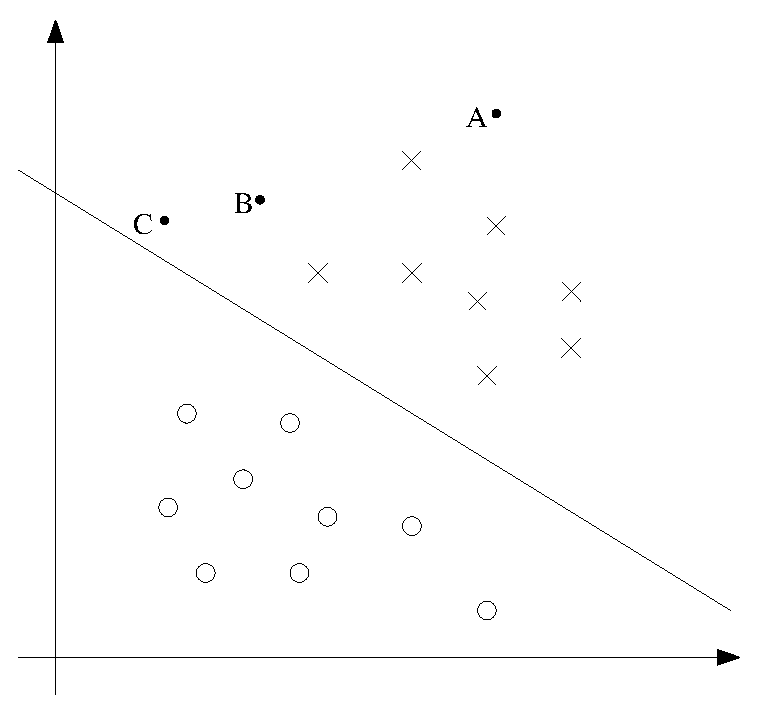
\includegraphics[scale=0.5]{geometricMargin1.eps}
\end{center}

Notice that the point A is very far from the decision boundary.  If we are asked to make a prediction
for the value of $y$ at A, it seems we should be quite confident that $y=1$ there.
Conversely, the point C is very close to the decision boundary, and while it's on the
side of the decision boundary on which we would predict $y=1$, it seems likely that just
a small change to the decision boundary could easily have caused out prediction to be $y=0$.
Hence, we're much more confident about our prediction at A than at C.  The point B lies
in-between these two cases, and more broadly, we see that if a point is far from the
separating hyperplane, then we may be significantly more confident in our predictions.
Again, informally we think it would be nice if, given a training set, we manage to find a
decision boundary that allows us to make all correct and confident (meaning far from the
decision boundary) predictions on the training examples.  We'll formalize this later using
the notion of geometric margins.


\section{Notation}

To make our discussion of SVMs easier, we'll first need to introduce a new notation
for talking about classification.
We will be considering a linear classifier for a binary
classification problem with labels $y$ and features $x$.  From now, we'll
use $y \in \{-1,1\}$ (instead of $\{0,1\}$) to denote the class labels.  Also, rather
than parameterizing our linear
classifier with the vector $\theta$, we will use parameters $w,b$, and write our
classifier as
\[
h_{w,b}(x) = g(w^Tx + b).
\]
Here, $g(z) = 1$ if $z \geq 0$, and $g(z) = -1$ otherwise.
This ``$w,b$'' notation allows us to explicitly treat the intercept term $b$ separately
from the other parameters.  (We also drop the convention we had previously of letting $x_0=1$ be
an extra coordinate in the input feature vector.)  Thus, $b$ takes the role of what was previously
$\theta_0$, and $w$ takes the role of $[\theta_1 \ldots \theta_{\di}]^T$.

Note also that, from our definition of $g$ above, our classifier will directly
predict either $1$ or $-1$ (cf. the perceptron algorithm), without first going through
the intermediate step of estimating $p(y=1)$ (which
is what logistic regression does).

\section{Functional and geometric margins}
	\label{margins}

Let's formalize the notions of the functional and geometric margins.  Given a training example
$(\xsi, \ysi)$, we define the {\bf functional margin} of $(w,b)$ with respect to the
training example as
\[
\hat\gamma^{(i)} = \ysi (w^T \xsi + b).
\]
Note that if $\ysi = 1$, then for the functional margin to be large (i.e., for our prediction
to be confident and correct), we need $w^T \xsi + b$ to be a large positive number.
Conversely, if $\ysi = -1$, then for the functional margin to be large, we need $w^T \xsi + b$
to be a large negative number.  Moreover, if
$\ysi (w^T \xsi + b) > 0$, then our prediction on this example is correct.  (Check this yourself.)
Hence, a large functional margin represents a confident and a correct prediction.

%The alert reader may have noticed one problem with the definition of the functional margin, however.
For a linear classifier with the choice of $g$ given above (taking values in $\{-1,1\}$),
there's one property of the functional margin that makes it not a very good measure of confidence,
however.  Given our choice of $g$, we note that if we replace $w$ with $2w$ and
$b$ with $2b$, then since
$g(w^Tx + b) = g(2w^Tx + 2b)$, this would not change $h_{w,b}(x)$ at all.  I.e., $g$, and hence
also $h_{w,b}(x)$, depends
only on the sign, but not on the magnitude, of $w^Tx+b$.  However, replacing $(w,b)$ with
$(2w,2b)$ also results in multiplying our functional margin by a factor of 2.  Thus, it seems
that by exploiting our freedom to scale $w$ and $b$, we can make the functional margin arbitrarily
large without really changing anything meaningful.  Intuitively, it might therefore make sense
to impose some sort of normalization condition such as that $||w||_2 = 1$; i.e., we might
replace $(w,b)$ with $(w/||w||_2,b/||w||_2)$, and instead consider the functional margin of
$(w/||w||_2,b/||w||_2)$.  We'll come back to this later.

Given a training set $S = \{(\xsi,\ysi);i=1,\ldots,\nexp\}$, we also define the function
margin of $(w,b)$ with respect to $S$ as the smallest of the functional margins of
the individual training examples.  Denoted
by $\hat\gamma$, this can therefore be written:
\[
\hat\gamma = \min_{i=1,\ldots,\nexp} \hat\gamma^{(i)}.
\]

Next, let's talk about {\bf geometric margins}.  Consider the picture below:

\begin{center}
% eps library outdated
% \epsfxsize=3in
% \epsffile{geometricMargin2.eps}
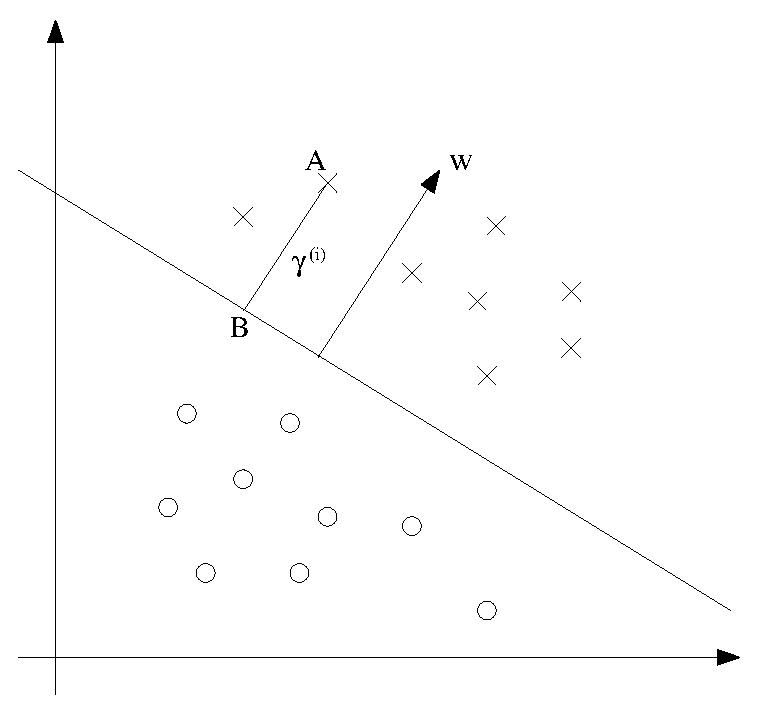
\includegraphics[scale=0.5]{geometricMargin2.eps}
\end{center}

The decision boundary corresponding to $(w,b)$ is shown, along with the vector $w$.  Note
that $w$ is orthogonal (at $90^\circ$) to the separating hyperplane.  (You should convince yourself
that this must be the case.)  Consider the point at A, which represents the input $\xsi$ of some
training example with label $\ysi=1$.  Its distance to the decision boundary, $\gsi$, is given
by the line segment AB.

How can we find the value of $\gsi$?  Well, $w/||w||$ is a unit-length vector pointing in the same
direction as $w$.
%The vector $\vec{AB}$ is therefore given by $\gsi w/||w||$, and since $A$ represents
%the point $\xsi$, we find
Since $A$ represents $\xsi$, we therefore find that the
point $B$ is given by $\xsi - \gsi \cdot w/||w||$.  But this point
lies on the decision boundary, and all points $x$ on the decision boundary satisfy the equation
$w^Tx + b = 0$.  Hence,
\[
w^T\left(\xsi - \gsi \frac{w}{||w||}\right) + b = 0.
\]
Solving for $\gsi$ yields
\[
\gsi = \frac{w^T\xsi + b}{||w||} = \left(\frac{w}{||w||}\right)^T\xsi + \frac{b}{||w||}.
\]
This was worked out for the case of a positive training example at A in the figure, where being
on the ``positive'' side of the decision boundary is good.  More generally, we define the geometric
margin of $(w,b)$ with respect to a training example $(\xsi, \ysi)$ to be
\[
\gsi = \ysi \left( \left(\frac{w}{||w||}\right)^T\xsi + \frac{b}{||w||} \right).
\]

Note that if $||w||=1$, then the functional margin equals the geometric margin---this thus gives
us a way of relating these two different notions of margin.  Also, the geometric margin
is invariant to rescaling of the parameters; i.e., if we replace $w$ with $2w$ and $b$ with $2b$, then
the geometric margin does not change.
%So, the geometric margin can also be thought of as a the
%functional margin with an additional normalization constraint.
This will in fact come in handy later.  Specifically, because of this invariance to the scaling of the parameters,
when trying to fit $w$ and $b$ to training data, we can impose an arbitrary scaling constraint on $w$ without
changing anything important; for instance, we can demand that $||w||=1$, or $|w_1| = 5$,
or $|w_1 + b| + |w_2| = 2$, and any of these can be satisfied simply by rescaling $w$ and $b$.

Finally, given a training set $S = \{(\xsi,\ysi); i=1,\ldots,\nexp\}$, we also define
the geometric margin of $(w,b)$ with respect to $S$ to be the smallest of the geometric margins on the
individual training examples:
\[
\gamma =\min_{i=1,\ldots,\nexp} \gamma^{(i)}.
\]

\section{The optimal margin classifier}

Given a training set, it seems from our previous discussion that a natural desideratum
is to try to find a decision boundary that maximizes the (geometric) margin, since this
would reflect a very confident set of predictions on the training set and a good ``fit'' to
the training data.  Specifically, this will result in a classifier that separates the positive
and the negative training examples with a ``gap'' (geometric margin).

For now, we will assume that we are given a training set that is linearly separable; i.e., that
it is possible to separate the positive and negative examples using some separating hyperplane.
How will we find the one that achieves the maximum geometric margin?  We can pose the following optimization
problem:
\begin{eqnarray*}
&\hbox{max}_{\gamma,w,b}& \gamma \\
&\;\;\;\;\;\;\;\hbox{s.t.}& \ysi (w^T\xsi + b) \geq \gamma,\;\; i=1, \ldots, \nexp \\
&& ||w|| = 1.
\end{eqnarray*}
I.e., we want to maximize $\gamma$, subject to each training example having functional margin at least $\gamma$.
The $||w||=1$ constraint moreover ensures that the functional margin equals to the geometric margin, so
we are also guaranteed that all the geometric margins are at least $\gamma$.
Thus, solving this problem will result in $(w,b)$ with the largest possible geometric margin
with respect to the training set.
%(Convince yourself that this is the right thing to do.)

If we could solve the optimization problem above, we'd be done.  But the ``$||w||=1$'' constraint is a nasty
(non-convex) one, and this problem certainly isn't in any format that we can plug into standard optimization
software to solve.  So, let's try transforming the problem into a nicer one. Consider:
\begin{eqnarray*}
&\hbox{max}_{\hat\gamma,w,b}& \frac{\hat\gamma}{||w||} \\
&\;\;\;\;\;\;\;\hbox{s.t.}& \ysi (w^T\xsi + b) \geq \hat\gamma,\;\; i=1, \ldots, \nexp
\end{eqnarray*}
Here, we're going to maximize $\hat\gamma/||w||$, subject to the functional margins all
being at least $\hat\gamma$.  Since the geometric and functional margins are related by
$\gamma = \hat\gamma/||w|$, this will give us the answer we want.  Moreover, we've gotten
rid of the constraint $||w||=1$ that we didn't like.  The downside is that we now
have a nasty (again, non-convex) objective $\frac{\hat\gamma}{||w||}$ function; and,
we still don't have any off-the-shelf software that can solve this form of an optimization problem.

Let's keep going.  Recall our earlier discussion that we can add an arbitrary scaling constraint
on $w$ and $b$ without changing anything.  This is the key idea we'll use now.  We will introduce the scaling
constraint that the functional margin of $w,b$ with respect to the training set must be 1:
\[
\hat\gamma = 1.
\]
Since multiplying $w$ and $b$ by some constant results in the functional margin being multiplied
by that same constant, this is indeed a scaling constraint, and can be satisfied by rescaling $w,b$.
Plugging this into our problem above, and noting that maximizing
$\hat\gamma/||w||$ = $1/||w||$
is the
same thing as minimizing $||w||^2$, we now have the following optimization problem:
\begin{eqnarray*}
&\hbox{min}_{w,b}& \frac{1}{2} ||w||^2 \\
&\;\;\;\;\;\;\;\hbox{s.t.}& \ysi (w^T\xsi + b) \geq 1,\;\; i=1, \ldots, \nexp
\end{eqnarray*}

We've now transformed the problem into a form that can be efficiently solved.  The above is an
optimization problem with a convex quadratic objective and only linear constraints.  Its
solution gives us the {\bf optimal margin classifier}.  This optimization problem can
be solved using commercial quadratic programming (QP) code.\footnote{You may be familiar with
linear programming, which solves optimization problems that have linear objectives and
linear constraints.  QP software is also widely available, which allows convex quadratic
objectives and linear constraints.}

While we could call the problem solved here, what we will instead do is make a
digression to talk about Lagrange duality.  This will lead us to our optimization problem's
dual form, which will play a key role in allowing us to use kernels to get optimal
margin classifiers to work efficiently in very high dimensional spaces.  The dual form
will also allow us to derive an efficient algorithm for solving the above optimization
problem that will typically do much better than generic QP software.


\section{Lagrange duality (optional reading)}

Let's temporarily put aside SVMs and maximum margin classifiers, and talk about solving
constrained optimization problems.

Consider a problem of the following form:
\begin{eqnarray*}
&\hbox{min}_w& f(w) \\
&\;\;\;\;\;\;\;\hbox{s.t.}& h_i(w) = 0, \;\; i=1, \ldots, l.
\end{eqnarray*}
Some of you may recall how the method of Lagrange multipliers can be used to solve it.
(Don't worry if you haven't seen it before.)  In this method, we define
the {\bf Lagrangian} to be
\[
\calL(w,\beta) = f(w) + \sum_{i=1}^l \beta_i h_i(w)
\]
Here, the $\beta_i$'s are called the {\bf Lagrange multipliers}.  We would then find and
set $\calL$'s partial derivatives to zero:
\[
\frac{\partial\calL}{\partial w_i} = 0; \;\;
\frac{\partial\calL}{\partial \beta_i} = 0,
\]
and solve for $w$ and $\beta$.
%Specifically, Lagrange proved that for $\wstar$ to be
%a solution to our optimization problem,

In this section, we will generalize this to constrained optimization problems in which we may
have inequality as well as equality constraints.  Due to time constraints, we won't really be
able to do the theory of Lagrange duality justice in this class,\footnote{Readers interested in learning more
about this topic are encouraged to read, e.g., R. T. Rockarfeller (1970), Convex Analysis,
Princeton University Press.} but we will give the main ideas and results, which we will then
apply to our optimal margin classifier's optimization problem.

Consider the following, which we'll call the {\bf primal} optimization problem:
\begin{eqnarray*}
&\hbox{min}_w& f(w) \\
&\;\;\;\;\;\;\;\hbox{s.t.}& g_i(w) \leq 0, \;\; i=1, \ldots, k \\
&& h_i(w) =  0, \;\; i=1, \ldots, l.
\end{eqnarray*}
To solve it, we start by defining the {\bf generalized Lagrangian}
\[
\calL(w,\alpha,\beta) = f(w) + \sum_{i=1}^k \alpha_i g_i(w) + \sum_{i=1}^l \beta_i h_i(w).
\]
Here, the $\alpha_i$'s and $\beta_i$'s are the Lagrange multipliers.
Consider the quantity
\[
\theta_\calP(w) = \max_{ \alpha, \beta\, :\, \alpha_i \geq 0 } \calL(w,\alpha,\beta).
\]
Here, the ``$\calP$'' subscript stands for ``primal.''  Let some $w$ be given.  If $w$ violates
any of the primal constraints (i.e., if either $g_i(w) > 0$ or $h_i(w) \neq 0$ for some $i$), then
you should be able to verify that
\begin{eqnarray}
\theta_\calP(w) &=& \max_{ \alpha, \beta\, :\, \alpha_i \geq 0 } f(w) + \sum_{i=1}^k \alpha_i g_i(w) + \sum_{i=1}^l \beta_i h_i(w) \\
&=& \infty.
\end{eqnarray}
Conversely, if the constraints are indeed satisfied for a particular value of $w$, then $\theta_\calP(w) = f(w)$. Hence,
\[
\theta_\calP(w) = \left\{ \begin{array}{ll} f(w)  & \hbox{if $w$ satisfies primal constraints} \\
					   \infty & \hbox{otherwise}. \end{array} \right.
\]
Thus, $\theta_\calP$ takes the same value as the objective in our problem for all values of $w$ that
satisfies the primal constraints, and is positive infinity if the constraints are violated.  Hence, if we
consider the minimization problem
\[
\min_w \theta_\calP(w) =
\min_w \max_{ \alpha, \beta\, :\, \alpha_i \geq 0 } \calL(w,\alpha,\beta),
\]
we see that it is the same problem (i.e., and has the same solutions as) our original, primal problem.
For later use, we also define the optimal value of the objective to
be $\pstar = \min_w \theta_\calP(w)$;
we call this the {\bf value} of the primal problem.

Now, let's look at a slightly different problem. We define
\[
\theta_\calD(\alpha, \beta) = \min_w \calL(w,\alpha,\beta).
\]
Here, the ``$\calD$'' subscript stands for ``dual.''  Note also that whereas in the
definition of $\theta_\calP$ we were optimizing (maximizing) with respect to $\alpha, \beta$,
here we are minimizing with respect to $w$.

We can now pose the {\bf dual} optimization problem:
\[
\max_{ \alpha, \beta\, :\, \alpha_i \geq 0 } \theta_\calD(\alpha, \beta) =
\max_{ \alpha, \beta\, :\, \alpha_i \geq 0 } \min_w \calL(w,\alpha,\beta).
\]
This is exactly the same as our primal problem shown above, except that the order of the
``$\max$'' and the ``$\min$'' are now exchanged.  We also define the optimal value of the
dual problem's objective to be $\dstar =
\max_{ \alpha, \beta\, :\, \alpha_i \geq 0 } \theta_\calD(w)$.

How are the primal and the dual problems related?  It can easily be shown that
\[
\dstar =
\max_{ \alpha, \beta\, :\, \alpha_i \geq 0 } \min_w \calL(w,\alpha,\beta) \leq
\min_w \max_{ \alpha, \beta\, :\, \alpha_i \geq 0 } \calL(w,\alpha,\beta) = \pstar.
\]
(You should convince yourself of this; this follows from the ``$\max \min$'' of a
function always being less than or equal to the ``$\min \max$.'')  However, under certain
conditions, we will have
\[
\dstar = \pstar,
\]
so that we can solve the dual problem in lieu of the primal problem.  Let's see what
these conditions are.

Suppose $f$ and the $g_i$'s are convex,\footnote{When $f$ has a Hessian, then it is convex if
and only if the Hessian is positive semi-definite.
For instance, $f(w) = w^Tw$ is convex; similarly, all linear (and affine) functions are
also convex.
(A function $f$ can also be convex without
being differentiable, but we won't need those more general definitions of convexity here.)}
and the $h_i$'s are affine.\footnote{I.e., there exists $a_i$, $b_i$, so that $h_i(w) = a_i^Tw + b_i$.
``Affine'' means the same thing as linear, except that we also allow the extra intercept term $b_i$.}
Suppose further that the constraints $g_i$ are (strictly) feasible; this means that there
exists some $w$ so that $g_i(w) < 0$ for all $i$.

Under our above assumptions, there must exist $\wstar, \alphastar, \betastar$ so that $\wstar$ is
the solution to the primal problem, $\alphastar, \betastar$ are the solution to the dual problem, and
moreover $\pstar = \dstar = \calL(\wstar, \alphastar,\betastar)$.  Moreover,
$\wstar, \alphastar$ and $\betastar$ satisfy the {\bf Karush-Kuhn-Tucker (KKT) conditions}, which are
as follows:
\begin{eqnarray}
\frac{\partial}{\partial w_i} \calL(\wstar,\alphastar,\betastar) &=& 0, \;\; i=1,\ldots, \di \label{eqn-kkt1} \\
\frac{\partial}{\partial \beta_i} \calL(\wstar,\alphastar,\betastar) &=& 0, \;\; i=1,\ldots, l \\
\alphastari g_i(\wstar) &=& 0, \;\; i=1,\ldots, k        \label{dual-complementarity}     \\
g_i(\wstar) &\leq& 0, \;\; i=1,\ldots, k \\
\alphastar  &\geq& 0, \;\; i=1,\ldots, k \label{eqn-kkt5}
\end{eqnarray}
Moreover, if some $\wstar, \alphastar, \betastar$ satisfy the KKT conditions, then it is also
a solution to the primal and dual problems.

We draw attention to Equation~(\ref{dual-complementarity}), which is called the
KKT {\bf dual complementarity} condition.  Specifically, it implies that if
$\alphastar_i > 0$, then $g_i(\wstar) = 0$.  (I.e., the ``$g_i(w) \leq 0$''
constraint is {\bf active}, meaning it holds with equality rather
than with inequality.)
Later on, this will be key for showing that the SVM has only a small number of ``support vectors'';
the KKT dual complementarity condition will also give us our convergence test when we talk
about the SMO algorithm.


\section{Optimal margin classifiers}

\notes{The equivalence of optimization problem~\eqref{eqn:primary} and the optimization problem~\eqref{eqn:dual}, and the relationship between the primary and dual variables in equation~\eqref{eqn-wdefinition} are the most important take home messages of this section. }

Previously, we posed the following (primal) optimization problem for finding the optimal margin
classifier:
\begin{eqnarray}
&\hbox{min}_{w,b}& \frac{1}{2} ||w||^2 \label{eqn:primary} \\
&\;\;\;\;\;\;\;\hbox{s.t.}& \ysi (w^T\xsi + b) \geq 1,\;\; i=1, \ldots, \nexp \nonumber
\end{eqnarray}
We can write the constraints as
\[
g_i(w) = - \ysi (w^T\xsi + b) + 1 \leq 0.
\]
We have one such constraint for each training example.  Note that from the KKT dual
complementarity condition, we will have $\alpha_i > 0$ only for the training examples
that have functional margin exactly equal to one (i.e., the ones corresponding
to constraints that hold with equality, $g_i(w) = 0$).  Consider the figure below,
in which a maximum margin separating hyperplane is shown by the solid line.

\begin{center}
% eps outdated
% \epsfxsize=3in
% \epsffile{supportVectors.eps}
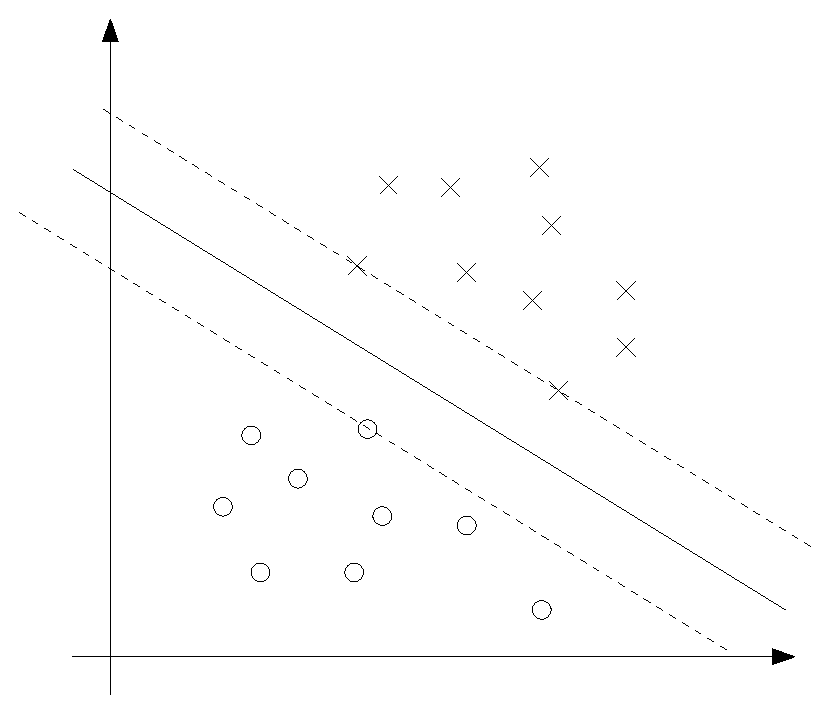
\includegraphics[scale=0.5]{supportVectors.eps}
\end{center}

The points with the smallest margins are exactly the ones closest to the decision
boundary; here, these are the three points (one negative and two positive examples)
that lie on the dashed lines parallel to the decision boundary.  Thus, only three
of the $\alpha_i$'s---namely, the ones corresponding to these three training examples---will
be non-zero at the optimal solution to our optimization problem.  These three points
are called the {\bf support vectors} in this problem. The fact that the number of
support vectors can be much smaller than the size the training set will be useful later.

Let's move on.  Looking ahead, as we develop the dual form of the problem, one key idea
to watch out for is that we'll try to write our algorithm in terms of only the inner product
$\langle x^{(i)}, x^{(j)} \rangle$ (think of this as $(x^{(i)})^T x^{(j)}$)
between points in the input feature space.  The fact that we can express our algorithm in
terms of these inner products will be key when we apply the kernel trick.

When we construct the Lagrangian for our optimization problem we have:
\begin{equation}
\calL(w,b,\alpha) = \frac{1}{2}||w||^2 - \sum_{i=1}^\nexp \alpha_i \left[ \ysi ( w^T\xsi + b) -1 \right].
			\label{eqn-lagrangian}
\end{equation}
Note that there're only ``$\alpha_i$'' but no ``$\beta_i$'' Lagrange multipliers, since
the problem has only inequality constraints.

Let's find the dual form of the problem.  To do so, we need to first minimize $\calL(w,b,\alpha)$ with
respect to $w$ and $b$ (for fixed $\alpha$), to get $\theta_\calD$, which we'll do by setting the
derivatives of $\calL$ with respect to $w$ and $b$ to zero.  We have:
\[
\nabla_w \calL(w,b,\alpha) = w- \sum_{i=1}^\nexp \alpha_i \ysi \xsi = 0
\]
This implies that
\begin{equation}
w = \sum_{i=1}^\nexp \alpha_i \ysi \xsi.	\label{eqn-wdefinition}
\end{equation}
As for the derivative with respect to $b$, we obtain
\begin{equation}
\frac{\partial}{\partial b} \calL(w,b,\alpha) = \sum_{i=1}^\nexp \alpha_i \ysi = 0. \label{eqn-bconstraint}
\end{equation}

If we take the definition of $w$ in Equation~(\ref{eqn-wdefinition}) and plug that back into
the Lagrangian (Equation~\ref{eqn-lagrangian}), and simplify, we get
\[
\calL(w,b,\alpha) = \sum_{i=1}^\nexp \alpha_i - \frac{1}{2} \sum_{i,j=1}^\nexp y^{(i)} y^{(j)} \alpha_i \alpha_j (x^{(i)})^T x^{(j)} - b\sum_{i=1}^\nexp \alpha_i \ysi.
\]
But from Equation~(\ref{eqn-bconstraint}), the last term must be zero, so we obtain
\[
\calL(w,b,\alpha) = \sum_{i=1}^\nexp \alpha_i - \frac{1}{2} \sum_{i,j=1}^\nexp y^{(i)} y^{(j)} \alpha_i \alpha_j (x^{(i)})^T x^{(j)}.
\]
Recall that we got to the equation above by minimizing $\calL$ with respect to $w$ and $b$.
Putting this together with the constraints $\alpha_i \geq 0$ (that we always had) and the
constraint (\ref{eqn-bconstraint}), we obtain the following dual optimization problem:
\begin{eqnarray}\label{eqn:dual}
&\hbox{max}_{\alpha} & W(\alpha) =
\sum_{i=1}^\nexp \alpha_i - \frac{1}{2} \sum_{i,j=1}^\nexp y^{(i)} y^{(j)} \alpha_i \alpha_j \langle x^{(i)},  x^{(j)} \rangle. \\
&\;\;\;\;\hbox{s.t.}& \alpha_i \geq 0, \;\; i=1,\ldots,\nexp \nonumber\\
&&                          \sum_{i=1}^\nexp \alpha_i \ysi = 0,\nonumber
\end{eqnarray}

You should also be able to verify that the conditions required for $\pstar = \dstar$ and the KKT conditions
(Equations~\ref{eqn-kkt1}--\ref{eqn-kkt5}) to hold are indeed satisfied in our optimization
problem. % (assuming that the training set is linearly separable).
Hence, we can solve the dual in lieu of solving the primal problem.  Specifically, in the dual problem
above, we have a maximization problem in which the parameters are the $\alpha_i$'s.  We'll talk later
about the specific algorithm that we're going to use to solve the dual problem, but if we are
indeed able to solve it (i.e., find the $\alpha$'s that maximize $W(\alpha)$ subject to the
constraints), then we can use Equation~(\ref{eqn-wdefinition}) to go back and find the optimal $w$'s
as a function of the $\alpha$'s.  Having found $\wstar$,
by considering the primal problem, it is also straightforward to find the optimal value for
the intercept term $b$ as
\begin{equation}
\bstar = - \frac{\max_{i : \ysi = -1} \wstar^T \xsi + \min_{i : \ysi = 1} \wstar^T \xsi}{2}.
		\label{eqn-bstar}
\end{equation}
(Check for yourself that this is correct.)

Before moving on, let's also take a more careful look at Equation~(\ref{eqn-wdefinition}), which gives
the optimal value of $w$ in terms of (the optimal value of) $\alpha$.  Suppose we've fit our
model's parameters
to a training set, and now wish to make a prediction at a new point input $x$.  We would then
calculate $w^Tx + b$, and predict $y=1$ if and only if this quantity is bigger than zero.  But
using~(\ref{eqn-wdefinition}), this quantity can also be written:
\begin{eqnarray}
w^Tx + b &=& \left(\sum_{i=1}^\nexp \alpha_i \ysi \xsi\right)^Tx + b \\
&=& \sum_{i=1}^\nexp \alpha_i \ysi \langle \xsi, x \rangle + b. \label{eqn-wtb}
\end{eqnarray}
Hence, if we've found the $\alpha_i$'s, in order to make a prediction, we have to calculate
a quantity that depends only on the inner product between $x$ and the points in
the training set.  Moreover, we saw earlier that the $\alpha_i$'s will all be zero except
for the support vectors.  Thus, many of the terms in the sum above will be zero, and we
really need to find only the inner products between $x$ and the support vectors (of
which there is often only a small number) in order calculate~(\ref{eqn-wtb}) and make our prediction.

By examining the dual form of the optimization problem,
we gained significant insight into the structure of the problem,
and were also able to write the entire algorithm in terms of only inner products between
input feature vectors.  In the next section, we will exploit this property to
apply the kernels to our classification problem.  The resulting algorithm, {\bf support vector machines},
will be able to efficiently learn in very high dimensional spaces.



\section{Regularization and the non-separable case (optional reading)}

The derivation of the SVM as presented so far assumed that the data is linearly separable.
While mapping data to a high dimensional feature space via $\phi$ does generally increase
the likelihood that the data is separable, we can't guarantee that it always will be so.
Also, in some cases it is not clear that finding a separating hyperplane is exactly what we'd want
to do, since that might
be susceptible to outliers.  For instance, the left figure below shows an optimal margin classifier,
and when a single outlier is added in the upper-left region (right figure), it causes the decision
boundary to make a dramatic swing, and the resulting classifier has a much smaller margin.

%\twofigboxnolabelFive{outlier.eps}{outlier2.eps}
\begin{center}
	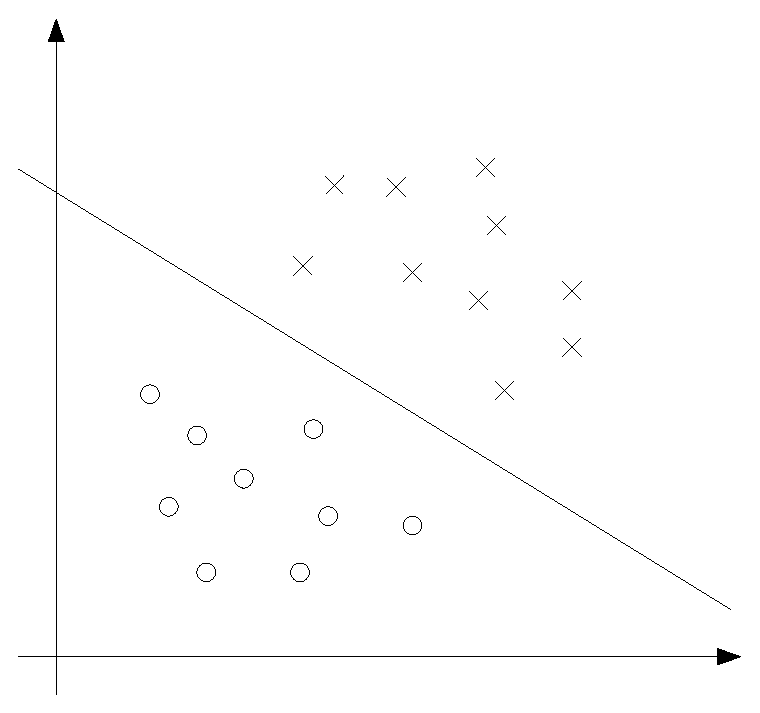
\includegraphics[width=.5\textwidth]{outlier.eps}\hfill
	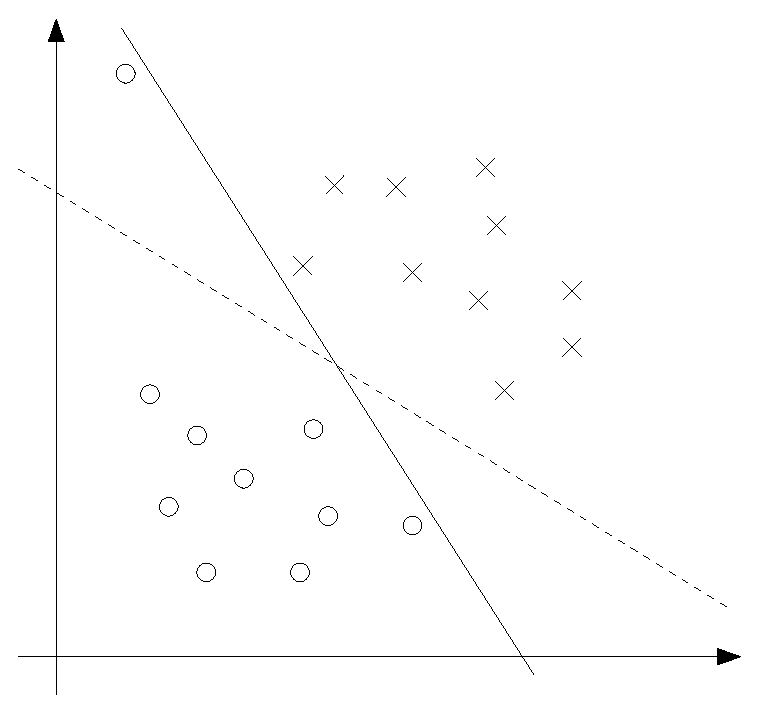
\includegraphics[width=.5\textwidth]{outlier2.eps}
\end{center}

To make the algorithm work for non-linearly separable datasets as well as be less sensitive
to outliers, we reformulate our optimization (using {\bf $\ell_1$ regularization}) as follows:
\begin{eqnarray*}
&\hbox{min}_{\gamma,w,b}& \frac{1}{2} ||w||^2  + C \sum_{i=1}^\nexp \xi_i \\
&\;\;\;\;\;\;\;\hbox{s.t.}& \ysi (w^T\xsi + b) \geq 1-\xi_i,\;\; i=1, \ldots, \nexp  \\
&& \xi_i \geq 0, \;\; i=1,\ldots,\nexp.
\end{eqnarray*}
Thus, examples are now permitted to have (functional) margin less than 1, and if an example
has functional margin $1-\xi_i$ (with $\xi > 0$), we would pay a cost of the objective function being
increased by $C\xi_i$.  The parameter $C$ controls the relative weighting between the
twin goals of making the $||w||^2$ small (which we saw earlier makes the margin large)
and of ensuring that most examples have functional margin at least 1.

As before, we can form the Lagrangian:
\[
\calL(w,b,\xi,\alpha,r) = \frac{1}{2} w^Tw + C \sum_{i=1}^\nexp \xi_i - \sum_{i=1}^\nexp \alpha_i \left[\ysi(x^Tw+b)-1+\xi_i\right] -  \sum_{i=1}^\nexp r_i \xi_i.
\]
Here, the $\alpha_i$'s and $r_i$'s are our Lagrange multipliers (constrained to be $\geq 0$).  We
won't go through the derivation of the dual again in detail, but after setting the derivatives with respect
to $w$ and $b$ to zero as before, substituting them back in, and simplifying, we obtain the
following dual form of the problem:
\begin{eqnarray*}
&\hbox{max}_{\alpha}& W(\alpha) =
\sum_{i=1}^\nexp \alpha_i - \frac{1}{2} \sum_{i,j=1}^\nexp y^{(i)} y^{(j)} \alpha_i \alpha_j \langle x^{(i)},  x^{(j)} \rangle \\
&\;\;\;\;\hbox{s.t.}& 0 \leq \alpha_i \leq C, \;\; i=1,\ldots,\nexp \\
&&                          \sum_{i=1}^\nexp \alpha_i \ysi = 0,
\end{eqnarray*}

As before, we also have that $w$ can be expressed in terms of the $\alpha_i$'s as given in
Equation~(\ref{eqn-wdefinition}), so that after solving the dual problem, we can continue to
use Equation~(\ref{eqn-wtb}) to make our predictions.  Note that, somewhat surprisingly, in
adding $\ell_1$ regularization, the only change to the dual problem is that what was
originally a constraint that $0 \leq \alpha_i$ has now become $0 \leq \alpha_i \leq C$.
The calculation for $\bstar$ also has to be modified (Equation~\ref{eqn-bstar} is no longer valid);
see the comments in the next section/Platt's paper.

Also, the KKT dual-complementarity conditions (which in the next section will be useful for testing
for the convergence of the SMO algorithm) are:
\begin{eqnarray}
\alpha_i = 0 &\rimp& \ysi(w^T\xsi + b) \geq 1  \label{eqn-l1kkt-1}\\
\alpha_i = C &\rimp& \ysi(w^T\xsi + b) \leq 1  \\
0 < \alpha_i < C &\rimp& \ysi(w^T\xsi + b) = 1.  \label{eqn-l1kkt-3}
\end{eqnarray}

Now, all that remains is to give an algorithm for actually solving the dual problem, which we
will do in the next section.

\section{The SMO algorithm (optional reading)}

The SMO (sequential minimal optimization) algorithm, due to John Platt, gives an efficient
way of solving the dual problem arising from the derivation of the SVM.  Partly to motivate
the SMO algorithm, and partly because it's interesting in its own right, let's first take
another digression to talk about the coordinate ascent algorithm.

\subsection{Coordinate ascent}

Consider trying to solve the unconstrained optimization problem
\[
\max_\alpha W(\alpha_1, \alpha_2, \ldots, \alpha_{\nexp}).
\]
Here, we think of $W$ as just some function of the parameters $\alpha_i$'s,
and for now ignore any relationship between this problem and SVMs.
We've already seen two optimization algorithms, gradient ascent and Newton's method.
% to be two algorithms for trying to solve this problem.
The new algorithm we're going to consider here is called {\bf coordinate ascent}:
\begin{enumerate}
\item[] Loop until convergence: $\{$
\item[] \begin{enumerate}
        \item[] For $i=1,\ldots,\nexp$, $\{$
\begin{enumerate} \item[] $\alpha_i := \arg \max_{\hat\alpha_i}
         W(\alpha_1, \ldots, \alpha_{i-1}, \hat\alpha_i, \alpha_{i+1}, \ldots, \alpha_{\nexp})$.
\end{enumerate}
\item[] $\}$
\end{enumerate}
\item[] $\}$
\end{enumerate}

Thus, in the innermost loop of this algorithm, we will hold all the variables except
for some $\alpha_i$ fixed, and reoptimize $W$ with respect to just the parameter $\alpha_i$.
In the version of this method presented here, the inner-loop reoptimizes the
variables in order $\alpha_1, \alpha_2, \ldots, \alpha_{\nexp}, \alpha_1, \alpha_2, \ldots$.
(A more sophisticated version might choose other orderings; for instance, we may
choose the next variable to update according to which one we expect to allow us to
make the largest
increase in $W(\alpha)$.)

When the function $W$ happens to be of such a form that the ``$\arg \max$''
in the inner loop can be performed efficiently, then coordinate ascent can be a fairly
efficient algorithm.  Here's a picture of coordinate ascent in action:

\begin{center}
% eps library outdated
% \epsfxsize=3in
% \epsffile{coordinateAscent.eps}
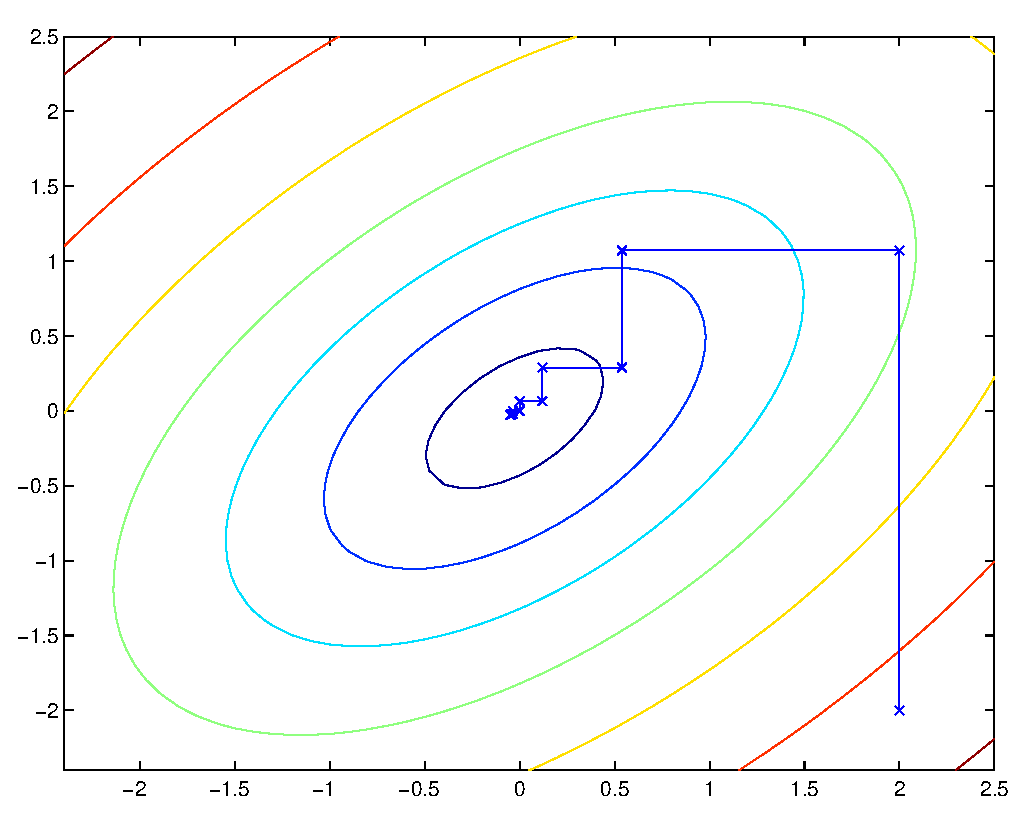
\includegraphics[scale=0.5]{coordinateAscent.eps}
\end{center}

The ellipses in the figure are the contours of a quadratic function that we want to optimize.
Coordinate
ascent was initialized at $(2,-2)$, and also plotted in the figure is the path that it took
on its way to the global maximum.  Notice that on each step, coordinate ascent takes a
step that's parallel to one of the axes, since only one variable is being optimized at a time.

\subsection{SMO}

We close off the discussion of SVMs by sketching the derivation of the SMO algorithm.
Some details will be left to the homework, and for others you may refer to the paper
excerpt handed out in class.
%\footnote{Extra copies can be picked up in the box outside Andrew's door.}

Here's the (dual) optimization problem that we want to solve:
\begin{eqnarray}
&\hbox{max}_{\alpha} & W(\alpha) =
\sum_{i=1}^\nexp \alpha_i - \frac{1}{2} \sum_{i,j=1}^\nexp y^{(i)} y^{(j)} \alpha_i \alpha_j \langle x^{(i)},  x^{(j)} \rangle. \\
&\;\;\;\;\hbox{s.t.}& 0 \leq \alpha_i \leq C, \;\; i=1,\ldots,\nexp \label{eqn-0cconstraint} \\
&&                          \sum_{i=1}^\nexp \alpha_i \ysi = 0.   \label{eqn-bconstraint2}
\end{eqnarray}

Let's say we have set of $\alpha_i$'s that satisfy the
constraints~(\ref{eqn-0cconstraint}-\ref{eqn-bconstraint2}).  Now, suppose we want to
hold $\alpha_2, \ldots, \alpha_{\nexp}$ fixed, and take a coordinate ascent step and reoptimize
the objective with respect to $\alpha_1$.  Can we make any progress?  The answer is no, because the
constraint~(\ref{eqn-bconstraint2}) ensures that
\[
\alpha_1 y^{(1)} = -\sum_{i=2}^\nexp \alpha_i \ysi.
\]
Or, by multiplying both sides by $y^{(1)}$, we equivalently have
\[
\alpha_1 = - y^{(1)} \sum_{i=2}^\nexp \alpha_i \ysi.
\]
(This step used the fact that $y^{(1)} \in \{-1, 1\}$, and hence $(y^{(1)})^2 = 1$.)  Hence,
$\alpha_1$ is exactly determined by the other $\alpha_i$'s, and if we were to
hold $\alpha_2,\ldots, \alpha_{\nexp}$ fixed, then we can't make any change to $\alpha_1$ without
violating the constraint~(\ref{eqn-bconstraint2}) in the optimization problem.

Thus, if we want to update some subject of the $\alpha_i$'s, we must update at least
two of them simultaneously in order to keep satisfying the constraints.  This motivates
the SMO algorithm, which simply does the following:

\begin{itemize}
\item[] Repeat till convergence $\{$
  \begin{enumerate}
  \item Select some pair $\alpha_i$ and $\alpha_j$ to update next (using a heuristic that tries
         to pick the two that will allow us to make the biggest progress towards the global maximum).
  \item Reoptimize $W(\alpha)$ with respect to  $\alpha_i$ and $\alpha_j$, while holding all
the other $\alpha_k$'s ($k\neq i,j$) fixed.
  \end{enumerate}
\item[] $\}$
\end{itemize}

To test for convergence of this algorithm, we can check whether the KKT conditions
(Equations~\ref{eqn-l1kkt-1}-\ref{eqn-l1kkt-3}) are satisfied to within some $\tol$.
Here, $\tol$ is the convergence tolerance parameter, and is typically set to
around 0.01 to 0.001.  (See the paper and pseudocode for details.)

%\begin{eqnarray}
%\alpha_i = 0 &\rimp& \ysi(w^T\xsi + b) \geq 1  \label{eqn-l1kkt-1}\\
%\alpha_i = C &\rimp& \ysi(w^T\xsi + b) \leq 1  \\
%0 < \alpha_i < C &\rimp& \ysi(w^T\xsi + b) = 1.  \label{eqn-l1kkt-3}
%\end{eqnarray}

The key reason that SMO is an efficient algorithm is that the update
to $\alpha_i$, $\alpha_j$ can be computed very efficiently.
Let's now briefly sketch the main ideas for deriving the efficient update.

Let's say we currently have some setting of the $\alpha_i$'s that satisfy the
constraints~(\ref{eqn-0cconstraint}-\ref{eqn-bconstraint2}), and suppose we've
decided to hold $\alpha_3, \ldots, \alpha_{\nexp}$ fixed, and want to reoptimize
$W(\alpha_1, \alpha_2, \ldots, \alpha_{\nexp})$ with respect to $\alpha_1$ and $\alpha_2$ (subject
to the constraints).  From~(\ref{eqn-bconstraint2}), we require that
\[
\alpha_1 y^{(1)} + \alpha_2 y^{(2)} = - \sum_{i=3}^\nexp \alpha_i y^{(i)}.
\]
Since the right hand side is fixed (as we've fixed $\alpha_3, \ldots \alpha_{\nexp}$), we
can just let it be denoted by some constant $\zeta$:
\begin{equation}
\alpha_1 y^{(1)} + \alpha_2 y^{(2)} = \zeta.		\label{eqn-alpha1}
\end{equation}
We can thus picture the constraints on $\alpha_1$ and $\alpha_2$ as follows:
\begin{center}
% eps library outdated
% \epsfxsize=3in
% \epsffile{alphaConstraints.eps}
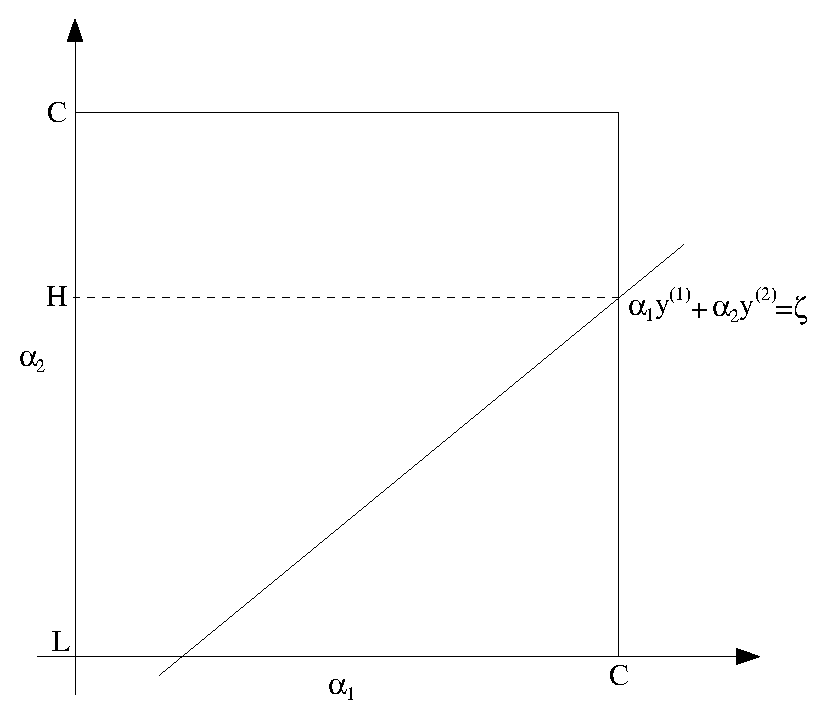
\includegraphics[scale=0.5]{alphaConstraints.eps}
\end{center}
From the constraints~(\ref{eqn-0cconstraint}), we know that $\alpha_1$ and $\alpha_2$ must
lie within the box $[0,C]\times [0,C]$ shown.  Also plotted is the line
$\alpha_1 y^{(1)} + \alpha_2 y^{(2)} = \zeta$, on which we know
$\alpha_1$ and $\alpha_2$ must lie.  Note also that, from these constraints,
we know $L \leq \alpha_2 \leq H$; otherwise, $(\alpha_1, \alpha_2)$ can't simultaneously
satisfy both the box and the straight line constraint.  In this example, $L=0$. But depending on
what the line $\alpha_1 y^{(1)} + \alpha_2 y^{(2)} = \zeta$ looks like,
this won't always necessarily be the case; but more generally, there will be
some lower-bound $L$ and some upper-bound $H$ on the permissible
values for $\alpha_2$ that will ensure that $\alpha_1$, $\alpha_2$ lie
within the box $[0,C] \times [0,C]$.

Using Equation~(\ref{eqn-alpha1}), we can also write $\alpha_1$ as a
function of $\alpha_2$:
\[
\alpha_1  = (\zeta - \alpha_2 y^{(2)})y^{(1)}.
\]
(Check this derivation yourself; we again used the fact that
$y^{(1)} \in \{-1,1\}$ so that $(y^{(1)})^2=1$.) Hence, the objective $W(\alpha)$ can
be written
\[
W(\alpha_1, \alpha_2, \ldots, \alpha_{\nexp}) =
W( (\zeta - \alpha_2 y^{(2)})y^{(1)}, \alpha_2, \ldots, \alpha_{\nexp}).
\]
Treating $\alpha_3, \ldots, \alpha_{\nexp}$ as constants, you should be able to verify that
this is just some quadratic function in $\alpha_2$.  I.e., this can also be expressed
in the form $a \alpha_2^2 + b \alpha_2 + c$ for some appropriate $a$, $b$, and $c$.
If we ignore the ``box'' constraints~(\ref{eqn-0cconstraint}) (or, equivalently, that
$L \leq \alpha_2 \leq H$), then we can easily maximize this quadratic function
by setting its derivative to zero and solving.  We'll let $\alpha_2^{\mathit new, unclipped}$
denote the resulting value of $\alpha_2$.  You should also be able to convince yourself
that if we had instead wanted to maximize $W$ with respect to $\alpha_2$ but subject to
the box constraint, then we can find the resulting value optimal simply by taking
$\alpha_2^{\mathit new, unclipped}$ and ``clipping'' it to lie in the $[L,H]$ interval,
to get
\begin{eqnarray*}
\alpha_2^{\textit new} &=& \left\{\begin{tabular}{ll}
         $H$                           & if $\alpha_2^{\textit new, unclipped} > H$  \\
         $\alpha_2^{\textit new, unclipped}$ & if $L \leq \alpha_2^{\textit new, unclipped} \leq H$  \\
         $L$                           & if $\alpha_2^{\textit new, unclipped} < L$
         \end{tabular} \right.  \\
\end{eqnarray*}
Finally, having found the $\alpha_2^{\mathit new}$, we can use Equation~(\ref{eqn-alpha1})
to go back and find the optimal value of $\alpha_1^{\mathit new}$.

There're a couple more details that are quite easy but that we'll leave you
to read about yourself in Platt's paper:  One is the choice of the heuristics used
to select the next $\alpha_i$, $\alpha_j$ to update; the other is how to
update $b$ as the SMO algorithm is run.

%This completes our discussion of the SMO algorithm.

%\section{End remarks}
%
%These notes have presented quite a long and mathematically involved story, but you now know about
%support vector machines and kernels---two very powerful ideas in machine learning.  Congratulations!

%# Nello Cristianini and John Shawe-Taylor. An Introduction to Support Vector Machines. Cambridge University Press, Cambridge, UK, 2000.

%# Bernhard Schölkopf, Chris Burges, and Alex Smola (eds). Advances in kernel Methods - Support Vector Learning. MIT Press, Cambridge, MA, 1999.

%# Bernhard Schölkopf and Alex Smola. Learning with kernels. MIT Press, Cambridge, MA, 2002.



%nbegin{center}
%\epsfxsize=3in
%\epsffile{foo.eps}
%\end{center}

\end{document}


